\documentclass[tikz,border=10pt]{standalone}
% Scale: s = 0.011976 cm/px (longest side ~8 cm); y flipped about y_px = 432
\begin{document}
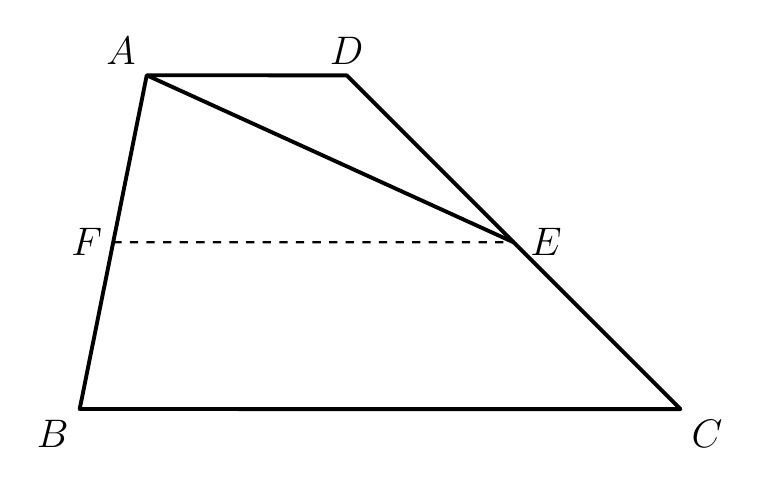
\begin{tikzpicture}[line width=1.4pt, line join=round]
  % Named coordinates (converted from pixels; unchanged)
  \coordinate (A) at (1.4604940687317445,4.238917604128043);
  \coordinate (D) at (3.9993589601468256,4.238314103380266);
  \coordinate (B) at (0.609045910532791,0.0004563781322062255);
  \coordinate (C) at (8.23819576075363,-0.0013571085379249226);
  \coordinate (E) at (6.119475555488799,2.117780164943525);
  \coordinate (F) at (1.0346297443462085,2.1189888579538843);

  % Solid trapezoid edges and diagonal-like segment A-E
  \draw (A) -- (D) -- (C) -- (B) -- cycle;
  \draw (A) -- (E);

  % Dashed segment F-E: lighter stroke, 3pt on / 3pt off dashes
  \draw[line width=0.8pt, dash pattern=on 3pt off 3pt] (F) -- (E);

  % Labels (14 pt font from cap-height metrics)
  \node[above left] at (A) {\fontsize{14}{16.8}\selectfont $A$};
  \node[above] at (D) {\fontsize{14}{16.8}\selectfont $D$};
  \node[below left] at (B) {\fontsize{14}{16.8}\selectfont $B$};
  \node[below right] at (C) {\fontsize{14}{16.8}\selectfont $C$};
  % E: directly right of the vertex, level with it, small 2pt xshift
  \node[right, xshift=2pt] at (E) {\fontsize{14}{16.8}\selectfont $E$};
  \node[left] at (F) {\fontsize{14}{16.8}\selectfont $F$};
\end{tikzpicture}
\end{document}
% GEOAGENT_REPAIR_V1 c18a466396f54661 bfbeff1f192d14d91174b4da4bd403f756ff276d8d05abb905377c2987759408
